% --- RSSM / PlaNet ---
% % --- Part C: RSSM (thread from Bierling 2025 Medium; figures from PlaNet PDF) ---
\begin{frame}[t]{RSSM: Motivation}
  \begin{itemize}\itemsep0.38em
    \item Purely deterministic RNNs (e.g., GRUs, LSTMs) struggle to represent multiple plausible futures in complex, stochastic environments.
    \item \textbf{Recurrent State Space Models (RSSM)} address this by combining:
      \begin{itemize}
        \item \textbf{Deterministic hidden state} $h_t$ (e.g., GRU): maintains long-term memory and context.
        \item \textbf{Stochastic state} $z_t$ (e.g., Gaussian): captures uncertainty and enables diverse possible futures.
      \end{itemize}
    \item This split allows RSSM to unify stable memory (for causality) and flexible modeling (for multi-modal, uncertain environments).
    \item Without the stochastic component, agents often \textbf{fail to learn} in partially observable or noisy tasks.
    \item Result: a flexible temporal representation for RL agents capable of handling uncertainty and representing many possible outcomes.
  \end{itemize}
\end{frame}

\begin{frame}[t]{RSSM: Architecture}
  \centering
  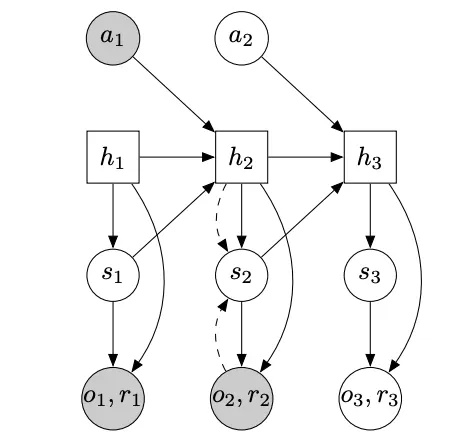
\includegraphics[width=0.65\linewidth,height=0.65\textheight,keepaspectratio]{assets/New-Lecture_World_Models/rssm_architecture_diagram.png}\\[0.2em]
  {\scriptsize Recurrent State Space model (RSSM). The filled circles are observed variables. Solid lines denote the generative process and dashed lines denote the inference model. Circles represent stochastic variables, squares represent deterministic variables. This is a mixed deterministic stochastic model Source: https://arxiv.org/pdf/1811.04551.}
\end{frame}

\begin{frame}[t]{RSSM: Dynamics}
  \begin{itemize}
    \item \textbf{Posterior transition (training):} Updates stochastic state using real observation 
    $$ z_t \sim q_\phi(z_t \mid h_t, x_t) $$
    \item \textbf{Prior transition (imagination):} Predicts next latent state without observation,
    $$ z_t \sim p_\theta(z_t \mid h_t) $$
    \item \textbf{Training objective:} Model learns by trying to reconstruct images, predict rewards, and making sure its imagined predictions match what really happened. Uses an loss (ELBO) that combines reconstruction, reward, and a KL-divergence.
    \item This ensures that planning in latent space is meaningful: predictions made during ``imagination'' are grounded in real transitions.
  \end{itemize}
\end{frame}
